\section{Struttura del file system}
    I dischi hanno costituito per molto tempo il più comune supporto di memorizzazione per grandi quantità di dati permanenti, e infatti qui sono spesso conservati i file systems. Sono adatti a questo scopo perché riscrivibili localmente, ossia possiamo prelevare, modificare e quindi riscrivere un blocco arbitrario, e perché possiamo accedere a qualsiasi blocco in qualsiasi momento, sia in maniera sequenziale che in modo diretto, il che funge bene da parallelo con l'accesso ai file che immaginiamo in un sistema elaborativo.
    
    Per migliorare le prestazioni dell'I/O, solitamente trasferimenti fra memoria centrale e dischi si eseguono per \textbf{blocchi}, che possono essere composti da diversi settori e sono spesso di 512 op 4096 byte.
    
    Spesso per presentare e manipolare questi dati si fa uso di uno o più \textbf{file system}. Abbiamo due problemi principali da trattare: il primo riguarda la presentazione dei dati all'utente, compresi attributi dei file e struttura delle directory. Il secondo tratta gli algoritmi impiegati per far corrispondere la struttura logica del file system a quella fisica del dispositivo di memorizzazione.
    
    Lo stesso file system, come illustrato dalla figura, è spesso composto da molti livelli distinti, ognuno dei quali si serve delle funzioni inferiori per crearne di più complesse, impiegate poi dai livelli superiori.
    
    \begin{figure}[h]
        \centering
        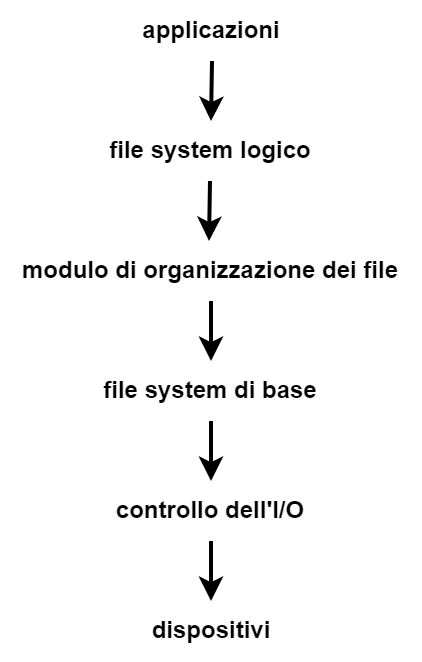
\includegraphics[width=0.35\textwidth]{img/img9.png}
        \caption{File system stratificato.}
        \label{fig:img9}
    \end{figure}
    
    \newpage
    
    Il livello più basso, il \textbf{controllo dell'I/O}, costituito semplicemente dei driver dei dispositivi e dai gestori dei segnali di interruzione, è impiegato per semplici scambi di informazioni fra memoria principale e secondaria. I driver dei dispositivi possono essere visti come traduttori che prendono in input istruzioni ad alto livello e le traducono in istruzioni adatte all'hardware, in base al controllore di I/O dedicato.
    
    Il \textbf{file system di base} deve solo inviare generici comandi all'appropriato dispositivo per leggere e scrivere blocchi fisici nel disco. Si occupa inoltre di gestire il buffer e la cache del file system. Il buffer contiene blocchi ancora da scrivere nel disco, e deve essere quindi esteso o svuotato quando si riempie, mentre la cache contiene metadati usati frequentemente dal file system, aumentandone le prestazioni. La gestione efficiente di queste due strutture risulta quindi piuttosto importante.
    
    Il modulo di \textbf{organizzazione dei file} è a conoscenza dei file e dei loro blocchi logici. Può quindi eseguire la traduzione da blocchi logici a fisici, che il livello inferiore dovrà poi trasferire, ricordando che mentre i blocchi logici sono numerati da $0$ a $1-n$, quelli fisici non rispettano una numerazione così ordinata. Questo modulo gestisce anche lo spazio libero.
    
    Infine, il \textbf{file system logico} gestisce i metadati; si tratta di tutto il contenuto del file system, eccetto gli effettivi dati contenuti nei file. Mantiene le strutture di file tramite i \textbf{blocchi di controllo dei file} (\textit{file control block}, FCB), detti \textbf{inode} nei file system UNIX, contenti informazioni sui file come la proprietà, i permessi, etc.
    
    Nei file system stratificati la duplicazione di codice è ridotta al minimo, in quanto si sfrutta molto il riuso di codice fra i vari file system. Purtroppo la stratificazione può generare un maggiore overhead del sistema operativo che può causare un decadimento delle prestazioni.
    
    Ad ogni modo la ricerca e lo sviluppo in campo di file system resta una questione aperta e ancora soggetti a customizzazioni problem-specific e miglioramenti.
    
\section{Operazioni del file system}
    Come detto in precedenza, per permettere l'accesso ai file i file system forniscono le chiamate \texttt{open()} e \texttt{close()}. Approfondiamo le strutture dati e le operazioni usate per realizzare le operazioni del file system.
    
    \subsection{Panoramica}
        Per realizzare i file system si utilizzano parecchie strutture dati, sia nei dischi sia in memoria. Sui dischi, il file system contiene informazioni su come avviare un sistema operativo memorizzato sul disco stesso, il numero totale di blocchi, il numero e la posizione dei blocchi liberi, la struttura delle directory e i singoli file.
        
        Fra le strutture presenti nei dischi troviamo tipicamente le seguenti.
        \begin{itemize}
            \item Il \textbf{blocco di controllo dell'avviamento} (\textit{boot control block}), che per ogni volume contiene informazioni utili all'avvio di un sistema operativo da quel volume; se il volume non contiene un sistema operativo, questo blocco può essere vuoto.
            
            \item Il \textbf{blocco di controllo del volume} (\textit{volume control block}); ciascuno di essi contiene i dettagli riguardanti il rispettivo volume, come il numero e la dimensione dei blocchi totali, liberi e i relativi puntatori.
            
            \item La \textbf{struttura della directory} (una per file system), usata per organizzare i file.
            
            \item Il \textbf{blocco di controllo del file} (FCB), contenente molti dettagli del relativo file.
        \end{itemize}
        
        Le informazioni tenute in memoria servono sia per la gestione del file system sia per migliorarne le prestazioni tramite l'uso di cache. I dati di caricano al momento del montaggio, si modificano durante l'utilizzo e si cancellano al momento dello smontaggio. Le strutture che vi possono essere incluse sono di vario tipo:
        \begin{itemize}
            \item La \textbf{tabella di montaggio} che contiene informazioni relative a ciascun volume montato.
            
            \item Una \textbf{cache della struttura della directory}, contenente le informazioni rilevanti relative alle directory cui i processi hanno avuto accesso recentemente.
            
            \item La \textbf{tabella di sistema dei file aperti}, contenente una copia dell'FCB per ciascun file aperto, insieme con altre informazioni.
            
            \item I \textbf{buffer} che conservano blocchi del file system durante la loro lettura o scrittura su disco.
        \end{itemize}
        
        Le applicazioni, per creare un nuovo file, eseguono una chiamata al file system logico, il quale conosce la struttura delle directory. Per creare un nuovo file, crea un nuovo FCB. Il sistema quindi carica in memoria e aggiorna la directory appropriata.
        
    \subsection{Utilizzo}
        Una volta creato un file, per essere usato per operazioni di I/O deve essere \textit{aperto}. La chiamata di sistema \texttt{open()} controlla innanzitutto se il file è già aperto, nel qual caso aggiunge un elemento alla tabella del processo che punta all'elemento corrispondente della tabella globale, metodo che fa risparmiare molto overhead da parte del sistema. In caso contrario apre il file nella tabella di sistema e punta a quest'ultimo dalla tabella del processo. Il nome dato all'elemento della tabella è detto \textit{file descriptor} in UNIX e \textit{file handle} in Windows.
        
        Quando un file viene invece chiuso la sua entry nella tabella dei file del processo viene eliminata e il contatore nella tabella di sistema viene decrementato. Ricordiamo che se questo contatore arriva a 0, la entry viene eliminata anche dalla tabella di sistema. Alcuni sistemi operativi complicano ulteriormente questo sistema, riadattando il file system per cose come connessioni di rete.
        
        Altra questione da non trascurare è quella dell'utilizzo delle \textbf{cache} quando possibile. Molti sistemi operativi hanno in cache tutti i metadati dei file aperti tranne i blocchi di dati effettivi.
        
\section{Realizzazione delle directory}
    Chiaramente la selezione di algoritmi di gestione delle directory ha un grande impatto sull'efficienza. Discutiamo ora i trade off di alcuni di questi algoritmi.
    
    \subsection{Lista lineare}
        Il concetto più semplice consiste nell'implementazione di una lista lineare che contiene i nomi dei file con puntatori ai blocchi dei dati. La sua esecuzione è tuttavia onerosa in termini di tempo. Per creare un file dobbiamo analizzare l'intera directory per verificare che non esista un file con lo stesso nome e accodare nel caso quello nuovo. Per la cancellazione dobbiamo scorrere nel caso peggiore l'intera directory per individuare il file da cancellare e fare lo shift degli elementi sulla destra.
        
        Alcuni semplici metodi di ottimizzazione comprendono il contrassegnare i file "liberi" anziché cancellarli, con un nome speciale o un bit di identificazione, oppure usare una lista concatenata per evitare lo shift degli elementi a destra dei cancellati.
        
        In generale il vero svantaggio di una lista è la ricerca dell'intera lista per trovare un file. L'utilizzo di una cache o l'impiego di una lista ordinata può ridurre l'overhead necessario, pur non risolvendo del tutto il problema.
        
    \subsection{Tabella hash}
        Abbiamo una tabella \textbf{hash} che prende in input un valore calcolato a partire dal nome dal file e restituisce un puntatore a un elemento della lista lineare contenente i puntatori dei file della directory.
        
        La ricerca, la creazione e la cancellazione di un file sono abbastanza semplici, anche se bisogna gestire i casi in cui si ottengono \textbf{collisioni}, ossia in cui due nomi di file diversi risultano nella stessa chiave.
        
        Il problema principale della tabella hash è la sua dimensione fissa e legata alla funzione hash. Se abbiamo una tabella di 64 elementi e la cui funzione può calcolare valori da 0 a 63. L'aggiunta di un 65esimo elemento implica l'estensione della tabella e il ricalcolo dei valori per una nuova funzione.
        
        Un'altra soluzione potrebbe essere l'avere gli elementi della tabella come teste di liste concatenate anziché singoli elementi. Questo è più lento perché richiede l'attraversamento di una lista in caso di collisioni, ma verosimilmente più efficiente di una semplice lista lineare.
        
\newpage
\section{Metodi di allocazione}
    La natura ad accesso diretto dei dischi li rende adatti ad accogliere file. Tuttavia ci sono diversi modi di allocare la memoria per i file in maniera più o meno efficiente. Esistono tre modi principali di farlo, che andremo qui a vedere. Chiaramente ognuno di essi presenta vantaggi e svantaggi. Alcuni sistemi dispongono di tutti e tre i modi, ma è più comune vederne uno solo su un singolo sistema.
    
    \subsection{Allocazione contigua}
        Questo metodo prevede l'occupazione di un insieme di blocchi \textbf{contigui} nel disco. In questo caso il numero di riposizionamenti della testina (\textit{seek}) per accedere a un singolo file è minimo. L'elemento di directory che descrive un file ne indica la posizione del primo blocco e la lunghezza, dai quali si può chiaramente ricavare la locazione dell'intero file.
        
        Questo metodo gestisce in modo semplice sia l'accesso sequenziale (basta accedere al primo blocco e ai $n$ successivi per lunghezza di $n$) che quello diretto (se vogliamo accedere al blocco $i$, e considerando il primo blocco indicato dalla entry della directory come $b$, ci basta accedere al blocco $b+i$).
        
        Un primo problema che troviamo con questa allocazione è l'individuazione dello spazio libero per un nuovo file, che non è immediata. Possiamo immaginare questo problema come una versione meno generale del problema dell'\textit{allocazione dinamica della memoria}, in cui dobbiamo soddisfare una richiesta di una certa dimensione data una lista di buchi liberi. Ricordiamo che i criteri più comuni di scelta di un buco libero sono \textit{best-fit} e \textit{first-fit}. Questi algoritmi soffrono della \textbf{frammentazione esterna}: lo spazio libero viene frammentato infatti in tanti piccoli buchi, che riuscirebbero ad accomodare un file (o molti file) se fossero contigui, ma non lo sono.
        
        Un metodo di \textbf{compattazione} sta nel trasferire tutti i file in un secondo file system e ricopiarli poi nello spazio libero lasciato nel primo in maniera contigua. Questo metodo funge effettivamente da deframmentazione, e spesso viene eseguito \textbf{off-line}, ossia con il file system non montato e quindi rende il sistema inutilizzabile. Oggi vari metodi di deframmentazione lasciano il sistema in uno stato utilizzabile ma a basse prestazioni.
        
        Un altro problema non da poco è l'allocazione dello spazio giusto per un file. Soprattutto per quanto riguarda file soggetti a una certa estensione, che devono per esempio contenere dati prodotti da un file, l'assegnazione di troppo spazio crea frammentazione, l'assegnazione di troppo poco spazio non gli permette di estendersi. La prima e poco desiderabile soluzione è terminare il programma utente con un appropriato messaggio di errore, il quale dovrà allocare più spazio e rieseguire il programma. L'altra soluzione consiste nel trovare un buco più grande, copiarvi il contenuto e rilasciare lo spazio previamente occupato.
        
        Anche conoscendo previamente lo spazio che un file andrà a occupare, il problema non viene risolto: se questo file cresce lentamente, durante la sua crescita ci sarà frammentazione interna.
        
        Alcuni sistemi operativi inizializzano un certo spazio in un primo momento e secondo necessità inseriscono poi una continuazione di questo spazio contiguo detta \textbf{estensione}. Il file si registrerà come il primo blocco, il numero di blocchi \textbf{e} la locazione del primo blocco della prossima estensione. Anche questa soluzione non è perfetta, in quanto le estensioni possono essere soggette a frammentazione esterna come i file originali.
        
    \subsection{Allocazione concatenata}
        Questo metodo risolve tutti i problemi dell'allocazione contigua. Il file è memorizzato come una lista concatenata che può essere sparsa in qualsiasi ordine sul disco. La directory contiene un puntatore al primo e all'ultimo blocco del file. Ogni blocco contiene chiaramente un puntatore al blocco successivo.
        
        Per creare un file, si crea semplicemente la entry nella directory che punta al primo blocco. Estendere il file consta semplicemente dell'atto di cercare il prossimo blocco vuoto tramite il sistema di gestione dello spazio libero e concatenarlo alla lista. La lettura è ancora più semplice, in quanto basta leggere i blocchi in sequenza. Questo metodo non implica nessun tipo di frammentazione esterna, e inoltre non richiede la computazione di nessuno spazio libero, in quanto il file può semplicemente continuare a crescere finché non vengono terminati i blocchi liberi.
        
        L'allocazione concatenata presenta comunque alcuni svantaggi. Quello principale sta nel fatto che può essere usata efficientemente solo nei file ad accesso sequenziale. Per trovare un arbitrario $i$-esimo blocco, occorre iniziare dal primo e percorrere $i$ blocchi. Su un HDD questo è oneroso in quanto la lettura del blocco successivo implica una lettura in memoria e talvolta il riposizionamento della testina.
        
        Un altro svantaggio sta nello spazio richiesto. Il puntatore al blocco successivo va memorizzato nel blocco, e se prendiamo per esempio puntatori dei 4 byte, lo 0,74\% del file è usato per memorizzare puntatori.
        
        La soluzione più comune a ciò consiste nel riunire più gruppi contigui di blocchi in \textbf{cluster}, e nell'allocare i cluster anziché i blocchi singoli. Essendo questa una via di mezzo fra i due metodi visti fino ad ora ne eredita parte dei vantaggi e degli svantaggi: mantiene la semplice corrispondenza fra memoria fisica e logica, aumenta il throughput rispetto all'allocazione concatenata in quanto richiede meno letture e riposizionamenti della testina, meno memoria è occupata per i puntatori, ma abbiamo allo stesso tempo più frammentazione interna. I cluster sono comunque molto impiegati nella realizzazione di file system in quanto possono ottimizzare l'accesso ai dischi in molti altri algoritmi.
        
        Un altro problema dell'allocazione concatenata è l'affidabilità. Siccome i file sono lunghe catene di blocchi tenuti insieme da puntatori sparsi per tutto il disco, si immagini cosa possa accadere qualora un puntatore andasse perduto o danneggiato. La lettura di un puntatore in maniera errata potrebbe causare la il collegamento alla lista dei blocchi liberi o di un altro file. Possibili soluzioni possono essere usare una lista doppiamente concatenata o la memorizzazione del nome del file e del relativo numero di blocco in ogni blocco; chiaramente questo aumenta considerevolmente sia spazio occupato da ogni file che overhead.
        
        Una variante importante del metodo di allocazione concatenata consiste nell'impiego della \textbf{tabella di allocazione dei file} (\textit{file allocation table}, FAT). Per contenere tale tabella si riserva parte dello spazio del disco all'interno di ogni volume; la FAT ha un elemento per ogni blocco del disco ed è indicizzata dal numero di blocco; si usa essenzialmente come una lista concatenata. L'elemento della directory contiene il numero del primo blocco del file. L'elemento della tabella così indicizzato contiene quindi il successivo e così via fino all'ultimo blocco che contiene un valore speciale di fine del file. I blocchi inutilizzati sono indicati nella tabella con il valore 0. L'allocazione di un nuovo blocco richiede semplicemente l'individuazione del primo blocco vuoto della tabella e la sostituzione di quel valore con l'inizio del blocco precedente.
        
    \subsection{Allocazione indicizzata}
        L'allocazione concatenata risolve i problemi della dichiarazione delle dimensioni del file e della frammentazione esterna presenti nel metodo di allocazione contigua. Tuttavia, senza la presenza di una FAT, l'allocazione concatenata soffre per quanto riguarda l'accesso diretto. L'\textbf{allocazione indicizzata} risolve questo problema raggruppando tutti i puntatori in un solo blocco: il \textbf{blocco indice}.
        
        Ogni file ha il proprio blocco indice: si tratta di un array di indirizzi di blocchi del disco: L'$i$-esimo elemento del blocco indice punta all'$i$-esimo blocco del file. La entry della directory contiene l'indirizzo del blocco indice. L'allocazione di nuovi blocchi consta semplicemente nel cercare il prossimo blocco impostato a \texttt{null} e riempirlo. La frammentazione esterna non sussiste e l'accesso diretto è intuitivo.
        
        Chiaramente per file molto piccoli, andiamo ad allocare un intero blocco indice, anche se quasi tutti i puntatori sono impostati a \texttt{null}, il che è uno spreco di memoria.
        
        Questo punto solleva la questione della dimensione del blocco indice. Un blocco troppo grande causa uno spreco di spazio (potrebbe essere quasi visto come frammentazione interna), mentre uno troppo piccolo potrebbe non riuscire a indicizzare tutti i blocchi del file. Fra i possibili meccanismi ci sono i seguenti:
        \begin{itemize}
            \item \textbf{Schema concatenato.} Possiamo immaginare più blocchi indice concatenati fra loro. Abbiamo un primo blocco piccolo che contiene il nome del file e i primi indirizzi, che può terminare con \texttt{null} o un puntatore all'inizio del prossimo blocco.
            
            \item \textbf{Indice a più livelli.} Questo meccanismo prevede la presenza di un primo indice che punta ad altri indici, i quali puntano ai blocchi del file. In base a necessità il numero di livelli potrebbe anche aumentare.
            
            \item \textbf{Schema combinato.} Un'altra possibilità, realizzata per esempio nei sistemi basati su UNIX, è quella di posizionare i primi blocchi effettivi nell'\textit{inode} del file. Se il file è molto piccolo, questo basta a memorizzare l'intero file. Altrimenti, l'ultimo blocco punterà a un blocco indice. Se quello basta bene, altrimenti il \textit{suo} ultimo blocco punterà a un blocco indice a due livelli, e così via. Andiamo quindi a diminuire la granularità della soluzione quando e solo se il file è di grandi dimensioni, avendo una soluzione adattiva.
        \end{itemize}
        
        Gli schemi di allocazione indicizzata soffrono di alcuni problemi di prestazioni che abbiamo visto nell'allocazione concatenata. In particolare, gli indirizzi sono tutti nello stesso blocco, ma i blocchi puntati potrebbero essere sparsi nel volume.